\section{Results}
\subsection{Summary}

     The algorithm was tested using three different datasets from \cite{sturm12iros}. The main contribution of the 
proposal is the filtering method, removing points that are unlikely to be present in the two point clouds and are not 
near edges extracted from the RGB image. For this reason, experiments were conducted to compare the whole system performance 
with and without filtering. In the three datasets the proposed method with filtering has significantly better performance after 
graph optimization. System was tested using only 100 frames to maintain accumulated error low, outliers detection and a more advanced  
pose graph optimization setup is necessary to work with more frames, but this topic is beyond the scope of this thesis.

\subsection{Quantitative Results}
\begin{center}
\begin{table}[H]
\begin{tabular}{ |l|c|c|}
\hline & filtered point cloud & full point cloud \\
\pbox{20cm}{RPE \\ (RMSE per second)} & 0.303387 m & 0.273217 m \\
\hline
\pbox{20cm} {RPE after graph optimization \\ (RMSE per second)} &  0.066331 m &  0.114962 m\\
\hline
\pbox{20cm}{ATE \\ (RMSE)} & 0.103475 m & 0.078300 m\\
\hline
\pbox{20cm} {ATE after graph optimization \\ (RMSE)} & 0.040286 m & 0.061566 m\\
\hline
\end{tabular}
\caption{freiburg1\_desk dataset (first 100 frames).}
\label{table:quantfd1}
\end{table}
\end{center}


\begin{center}
\begin{table}[H]
\begin{tabular}{ |l|c|c|}
\hline & filtered point cloud & full point cloud \\
\pbox{20cm} {RPE \\ (RMSE per second)} & 0.124113 m & 0.158429 m \\
\hline
\pbox{20cm}{RPE after graph optimization \\ (RMSE per second)} & 0.081823 m & 0.112310 m\\
\hline
\pbox{20cm} {ATE \\ (RMSE)} & 0.059671 m & 0.078372 m\\
\hline
\pbox{20cm} {ATE after graph optimization \\ (RMSE)} & 0.048461 m & 0.063755 m\\
\hline
\end{tabular}
\caption{freiburg1\_room dataset (first 100 frames).}
\label{table:quantroom}
\end{table}
\end{center}

\begin{center}
\begin{table}[H]
\begin{tabular}{ |l|c|c|}
\hline & filtered point cloud & full point cloud \\
\pbox{20cm}{RPE \\ (RMSE per second)} &  0.044770 m & 0.105270 m\\
\hline
\pbox{20cm} {RPE after graph optimization \\ (RMSE per second)} & 0.041990 m & 0.114090 m\\
\hline
\pbox{20cm} {ATE \\ (RMSE)} & 0.025618 m  & 0.056300 m\\
\hline
\pbox{20cm} {ATE after graph optimization \\ (RMSE)} & 0.026500 m & 0.057818 m \\
\hline
\end{tabular}
\caption{freiburg2\_desk dataset (first 100 frames).}
\label{table:quantfd2}
\end{table}
\end{center}

\begin{center}
\begin{figure}
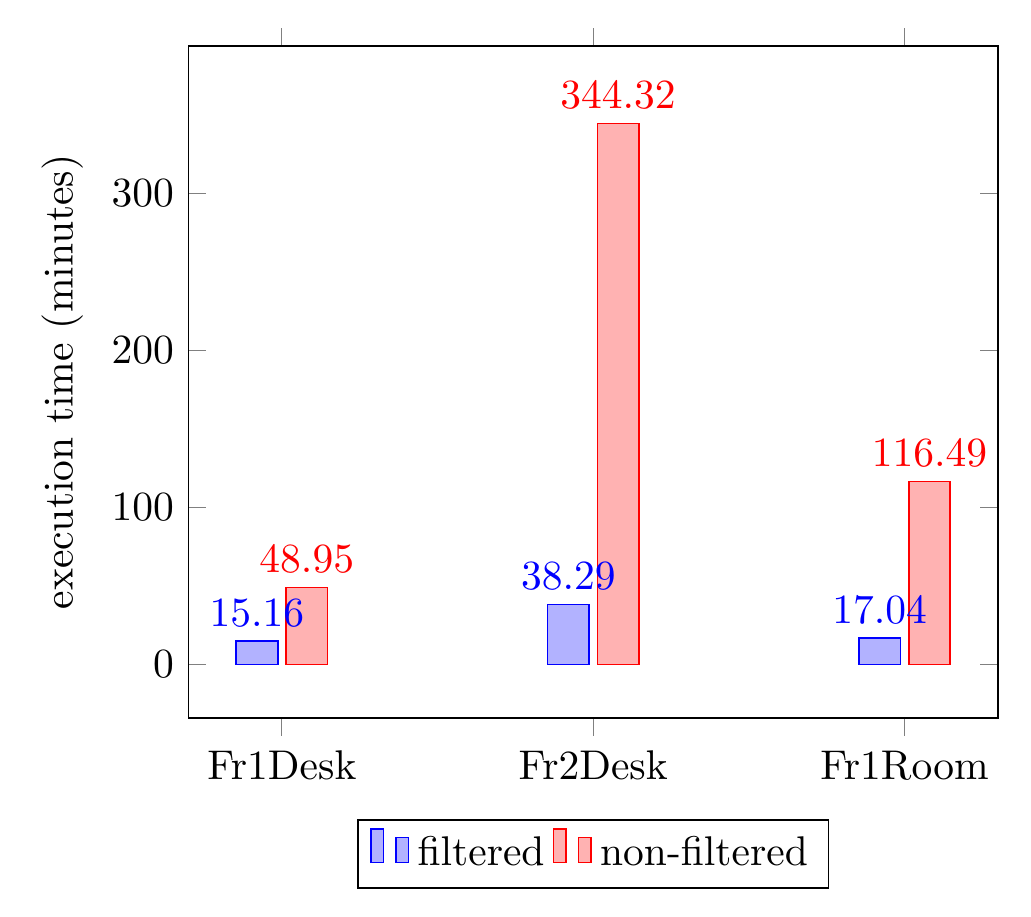
\begin{tikzpicture}[scale=1.5]
\begin{axis}[
    ybar,
    enlargelimits=0.15,
    legend style={at={(0.5,-0.15)},
      anchor=north,legend columns=-1},
    ylabel={execution time (minutes)},
    symbolic x coords={Fr1Desk,Fr2Desk,Fr1Room},
    xtick=data,
    nodes near coords,
    nodes near coords align={vertical},
    ]
\addplot coordinates {(Fr1Desk,15.16) (Fr2Desk,38.29) (Fr1Room,17.04)};
\addplot coordinates {(Fr1Desk,48.95) (Fr2Desk,344.32) (Fr1Room,116.49)};
\legend{filtered,non-filtered}
\end{axis}
\end{tikzpicture}
\caption{Average execution time with 100 frames in three different datasets} 
\end{figure}
\end{center}

In the freiburg1\_desk dataset before applying graph optimization better results where obtained using 
the full point cloud. This occurs because prior to graph optimization only consecutive frames are aligned, 
consecutive frames are more likely to have a small relative movement, making the alignment between two point clouds 
less prone to 
errors. When graph optimization is used, non consecutive frames are aligned in order to add restrictions to the graph, 
incrementing the difficulty of 
the alignment. Under this scenario the advantages of using the proposed filtering approach becomes clear.


\begin{figure}[H]
\begin{center}
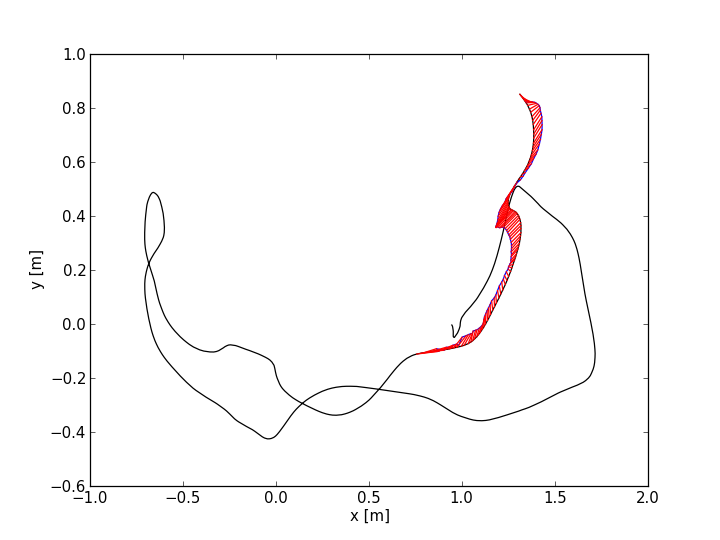
\includegraphics[scale=0.75]{images/freiburg1_desk_1_100_fullcloud_optimized.png}
\caption{freiburg1\_desk dataset first 100 frames: Obtained trajectory using full point cloud after graph optimization. Ground truth trajectory (black), estimated trajectory (blue) and difference (red).}
\label{fig:jan}
\end{center}
\end{figure}

\begin{figure}[H]
\begin{center}
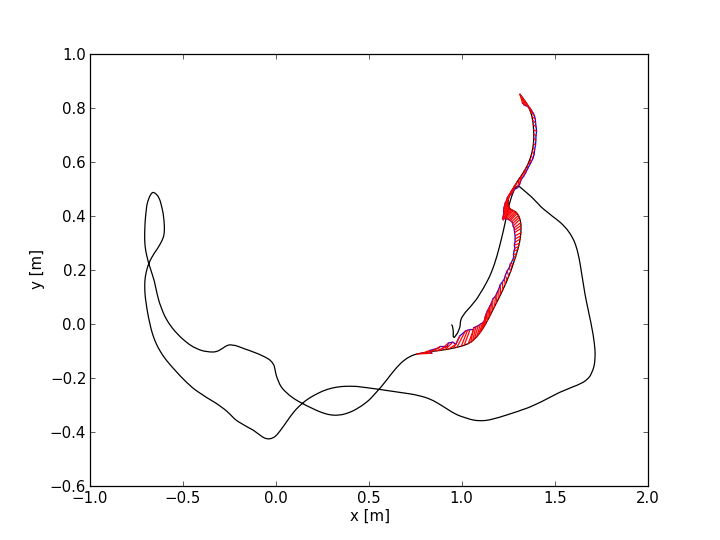
\includegraphics[scale=0.75]{images/freiburg1_desk_1_100_optimized.png}
\caption{freiburg1\_desk dataset first 100 frames: Obtained trajectory using point cloud filtered with proposed method after graph optimization. Ground truth trajectory (black), estimated trajectory (blue) and difference (red).}
\label{fig:jan}
\end{center}
\end{figure}

\begin{figure}[H]
\begin{center}
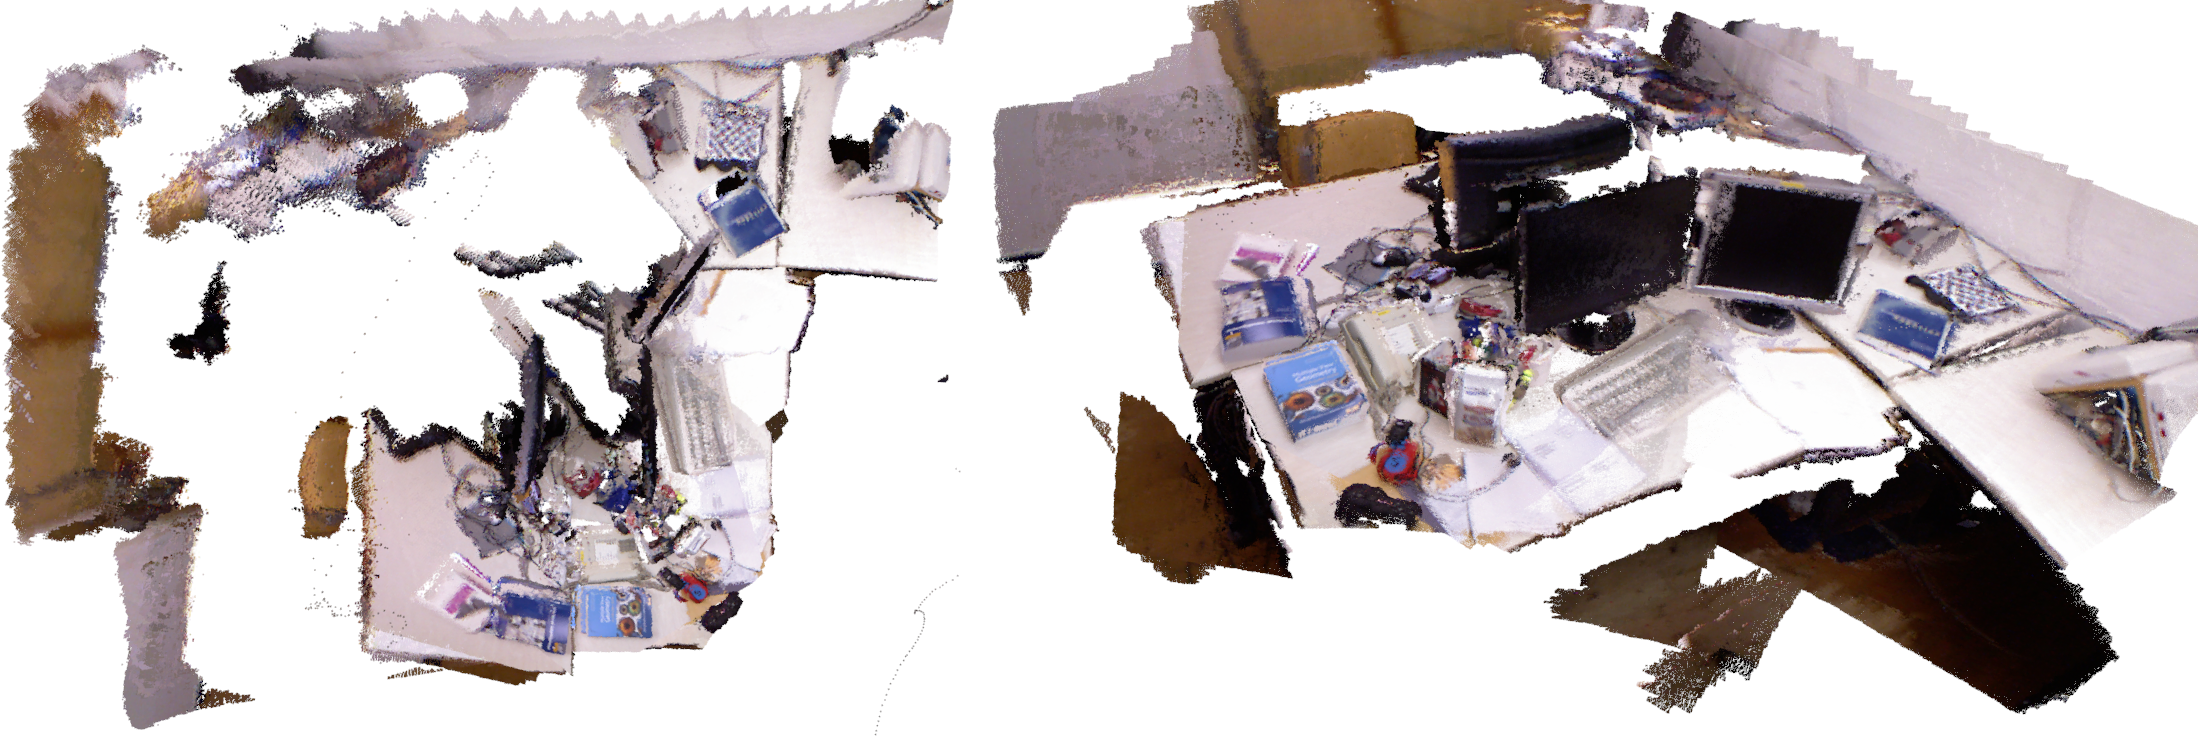
\includegraphics[scale=0.2]{images/freiburg1_desk.png}
\caption{freiburg1\_desk dataset registration of first 100 frames with proposed method. Point cloud downsampled using voxels of $35mm$.}
\label{fig:jan}
\end{center}
\end{figure}


\begin{figure}[H]
\begin{center}
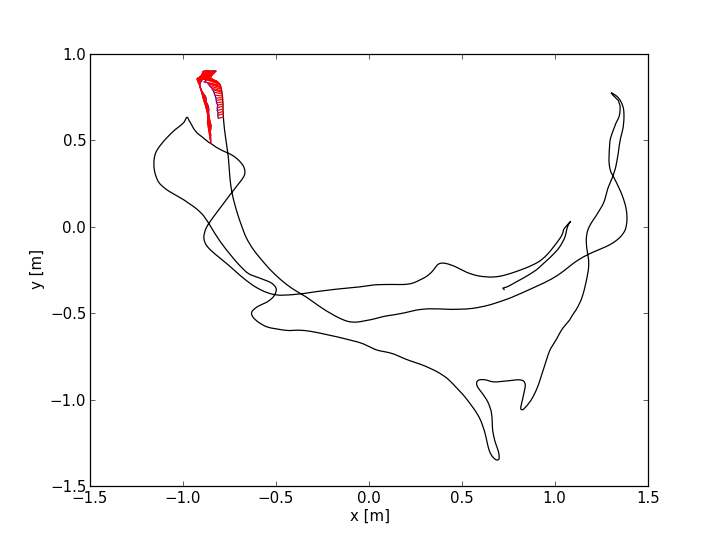
\includegraphics[scale=0.75]{images/freiburg1_room_1_100_fullcloud_optimized.png}
\caption{freiburg1\_room dataset first 100 frames: Obtained trajectory using full point cloud after graph optimization. Ground truth trajectory (black), estimated trajectory (blue) and difference (red).}
\label{fig:jan}
\end{center}
\end{figure}

\begin{figure}[H]
\begin{center}
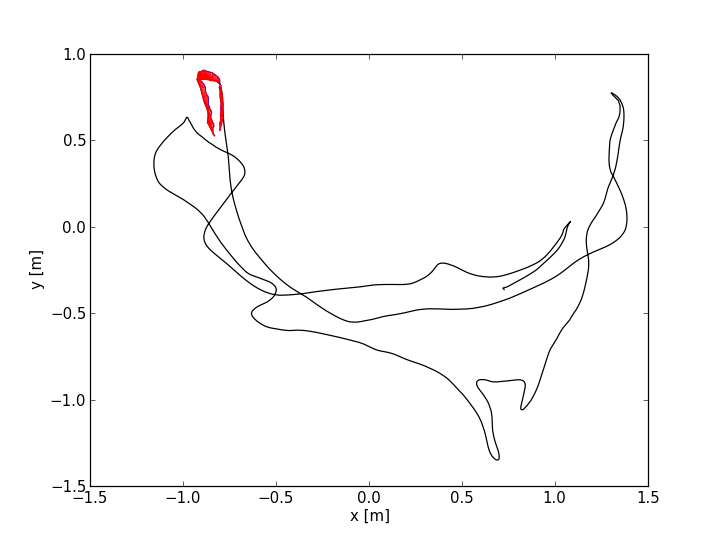
\includegraphics[scale=0.75]{images/freiburg1_room_1_100_optimized.png}
\caption{freiburg1\_room dataset first 100 frames: Obtained trajectory using point cloud filtered with proposed method after graph optimization. Ground truth trajectory (black), estimated trajectory (blue) and difference (red).}
\label{fig:jan}
\end{center}
\end{figure}

\begin{figure}[H]
\begin{center}
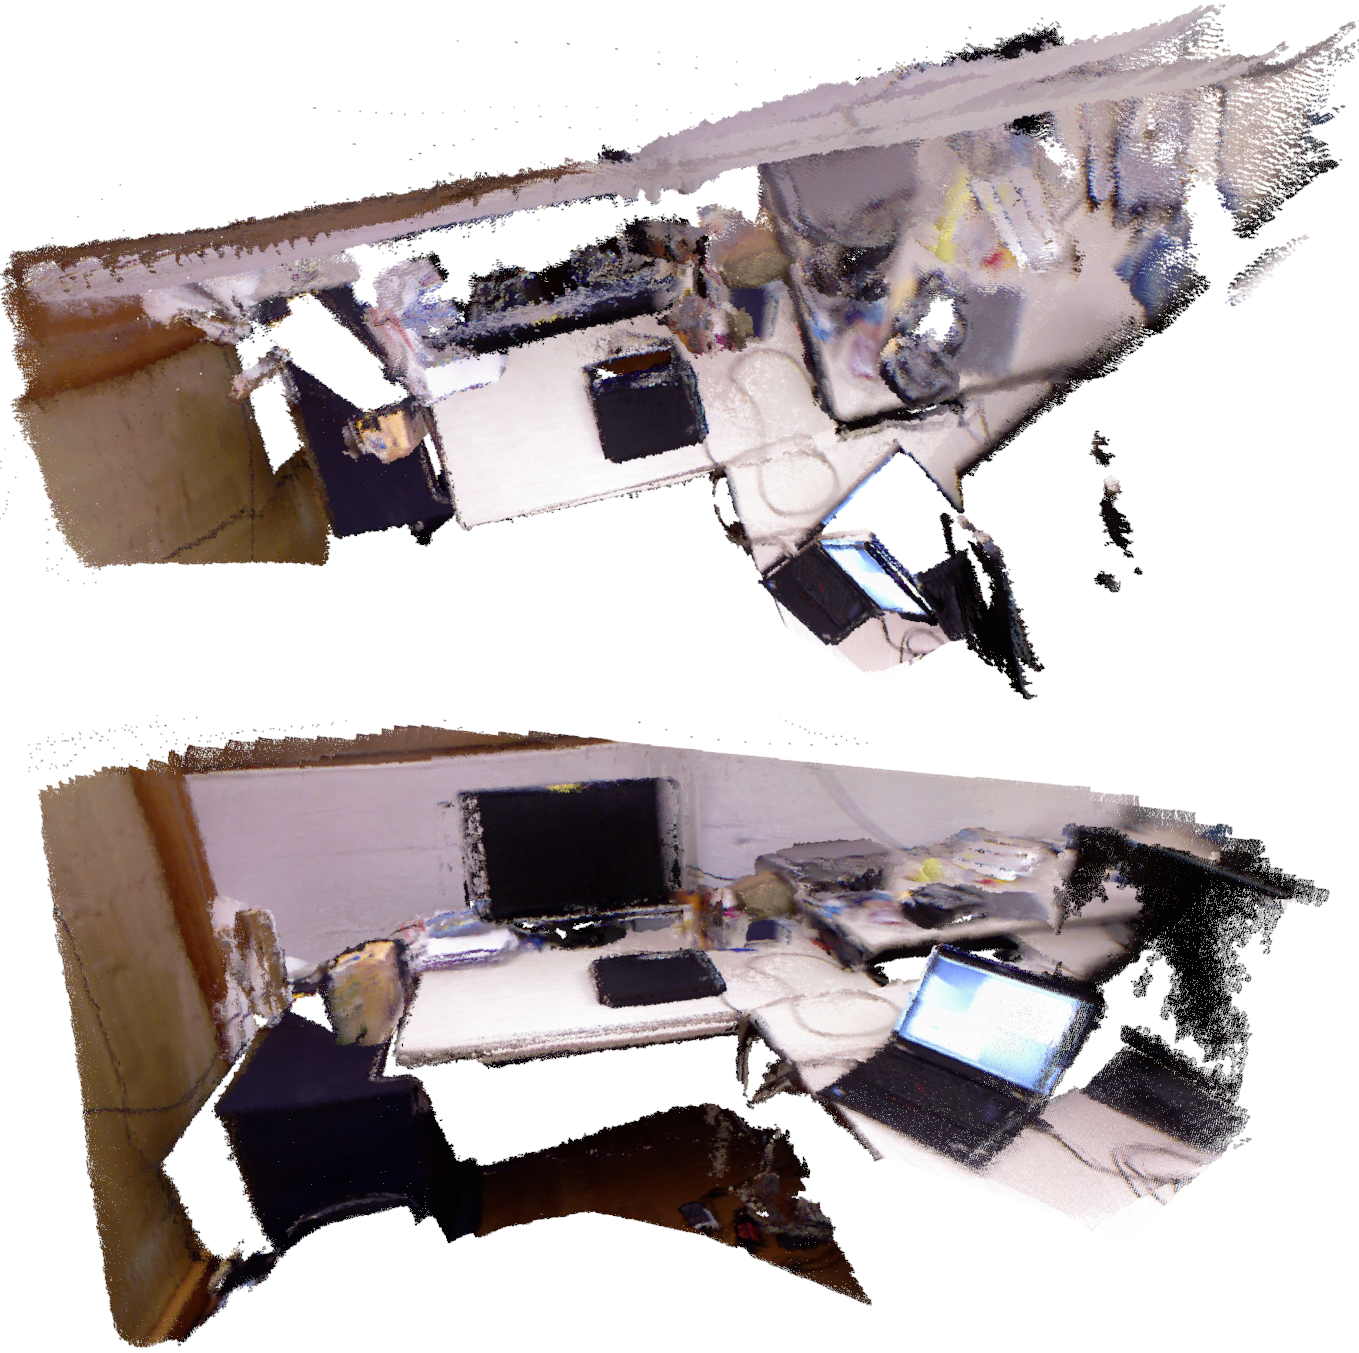
\includegraphics[scale=0.27]{images/freiburg1_room.png}
\caption{freiburg1\_room dataset registration of first 100 frames with proposed method. Point cloud downsampled using voxels of $35mm$.}
\label{fig:jan}
\end{center}
\end{figure}


\begin{figure}[H]
\begin{center}
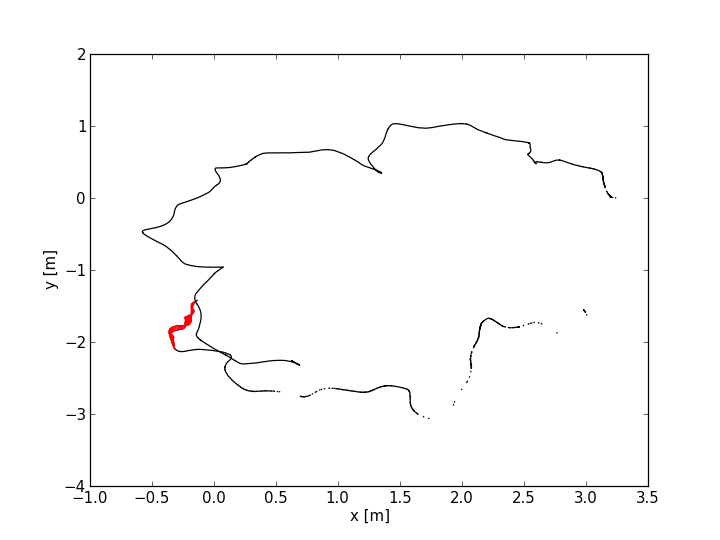
\includegraphics[scale=0.75]{images/freiburg2_desk_1_100_fullcloud_optimized.png}
\caption{freiburg2\_desk dataset first 100 frames: Obtained trajectory using full point cloud after graph optimization. Ground truth trajectory (black), estimated trajectory (blue) and difference (red).}
\label{fig:jan}
\end{center}
\end{figure}

\begin{figure}[H]
\begin{center}
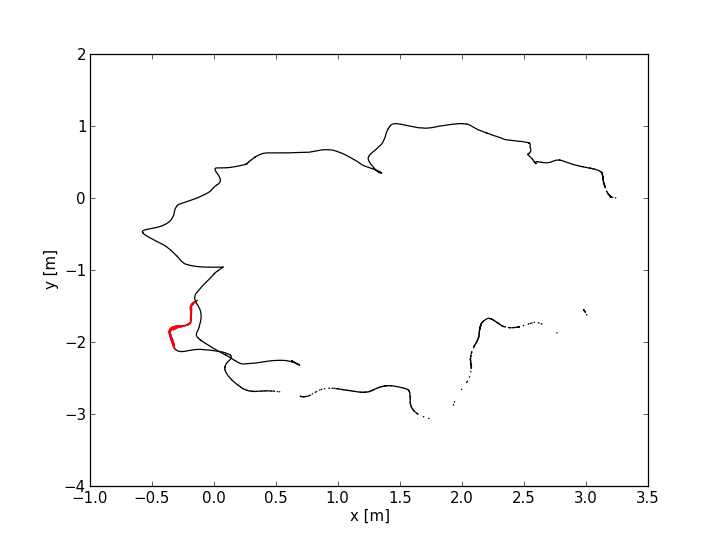
\includegraphics[scale=0.75]{images/freiburg2_desk_1_100_optimized.png}
\caption{freiburg2\_desk dataset first 100 frames: Obtained trajectory using point cloud filtered with proposed method after graph optimization. Ground truth trajectory (black), estimated trajectory (blue) and difference (red).}
\label{fig:jan}
\end{center}
\end{figure}


\begin{figure}[H]
\begin{center}
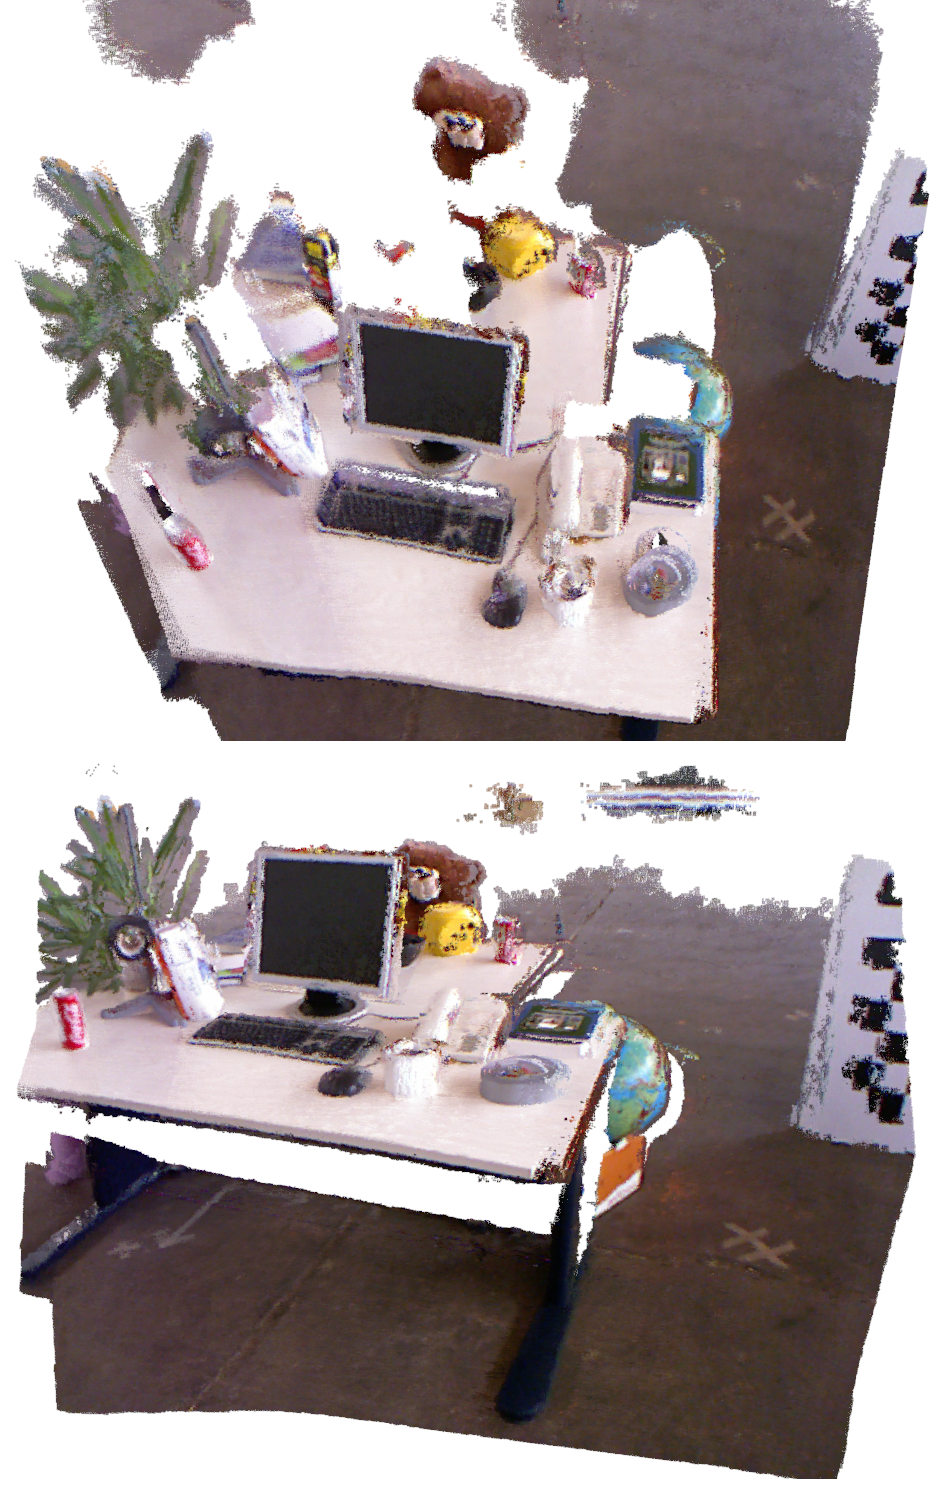
\includegraphics[scale=0.27]{images/freiburg2_desk.png}
\caption{freiburg2\_desk dataset registration of first 100 frames with proposed method. Point cloud downsampled using voxels of $55mm$.}
\label{fig:jan}
\end{center}
\end{figure}


As it can be seen in previous plots, when applying the proposed filtering to the point clouds, the trajectory of the sensor gets 
closer to ground truth. Better results are obtained working with a representative small subset of the original data and these results 
can be greatly improved with a better setup of the pose graph. Reconstructed scenes shown the potential of the method and the quantitative 
results can be verified through a visual inspection. 

The best results where obtained in the freiburg2\_desk dataset, possibly due to the visual richness of the images more clues where obtained 
to find the relative transformations.
